\documentclass[tikz,border=6pt]{standalone}
\usetikzlibrary{arrows.meta,calc,angles,quotes,decorations.markings}
\usepackage{tikz}                  % 主宏包
\usetikzlibrary{arrows.meta}       % 画箭头(Latex、Stealth等样式)
\usetikzlibrary{calc}              % 支持坐标计算 ($(A)!t!(B)$)
\usetikzlibrary{angles,quotes}     % 用于角度标记 \pic {...}
\usetikzlibrary{decorations.markings} % 绘制带标记或自定义箭头的线
\begin{document}
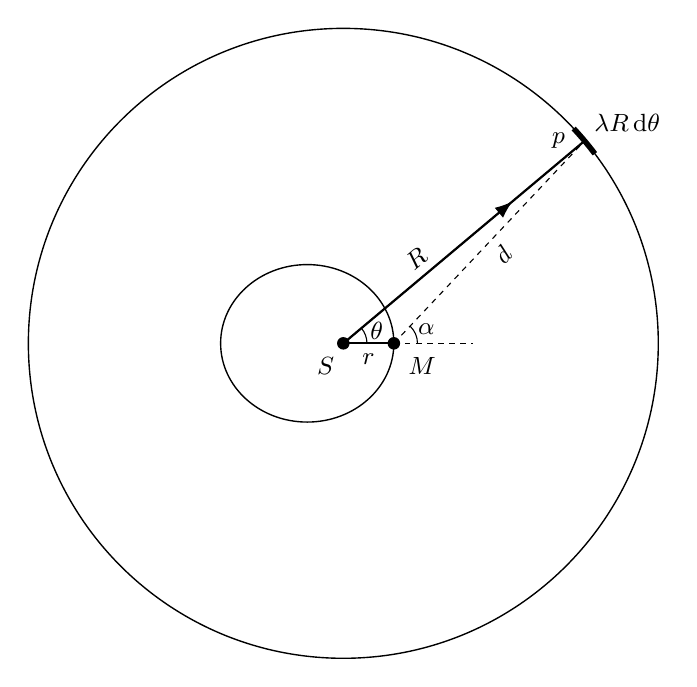
\begin{tikzpicture}[scale=1.0,
    dot/.style={circle,fill,inner sep=1.6pt},
    >={Latex[length=2.2mm]},
    angle/.style={draw,->,angle eccentricity=1.2,angle radius=9pt},
    faint/.style={dash pattern=on 2pt off 2pt},
    every node/.style={font=\small}
]

%------------------------ 基本参数(可按需改动) ------------------------
\def\R{4.0}              % 大圆半径
\def\a{1.1}              % 椭圆半长轴
\def\b{1}              % 椭圆半短轴
% 令圆心 S 同时为椭圆的一个焦点:c = sqrt(a^2-b^2),椭圆中心在 (c,0)
\pgfmathsetmacro{\c}{sqrt(\a*\a-\b*\b)}
\coordinate (S) at (0,0);
\coordinate (R) at (\R,0);

% 椭圆上一点参数角(几何参数,不是极角)
\def\t{0}  % 参数角
\pgfmathsetmacro{\Mx}{\a*cos(\t) - \c}
\pgfmathsetmacro{\My}{\b*sin(\t)}
\coordinate (M) at (\Mx,\My);

% 圆上的两点
\def\aPone{40}  % P1 在圆上的极角
\coordinate (P1) at ({\R*cos(\aPone)}, {\R*sin(\aPone)});

%------------------------ 绘制主体 ------------------------
% 大圆
\draw[line width=0.5pt] (S) circle (\R);

% 椭圆
\draw[line width=0.5pt] (-\c, 0) ellipse [x radius=\a, y radius=\b];

% 参考坐标轴
%\draw[faint] (0,-2) -- (0,2) node[above] {$y$};

% 连接线
\draw[thick] (S) -- (M) node[midway, below] {$r$};
\draw[thick] (P1) -- (S);
\draw[faint] (M) -- (P1) node[midway, below, sloped] {$d$};

% 水平/垂直虚线参考
\draw[faint] ($(M)+(0,0)$) -- ($(M)+(1.0,0)$);
%\draw[faint] ($(M)+(0,-0.9)$) -- ($(M)+(0,0.9)$);

% 点与标注
\node[dot,label={[xshift=2pt,yshift=0pt]below left:$S$}] at (S) {};
\node[dot,label=below right:$M$] at (M) {};
\node[label=left:$p$] at (P1) {};

%------------------------ 角度标记 ------------------------
% 在 S 处的极角 theta:取 x 轴正向与 SM 之间的角
\pic [draw, angle radius=0.3cm, angle eccentricity=1.5, "$\theta$"] {angle = R--S--P1};

% 可选:在 S 处再做 P1S 与 SM 夹角(小角 α)
\pic [draw, angle radius=0.3cm, angle eccentricity=1.5, "$\alpha$"] {angle = R--M--P1};

% 可选:在圆上 P1 处做很小的弧段并标注 \lambda R d\theta
\def\dt{3}
\draw[line width=2pt]
  let \p1=(P1), \n1={atan2(\y1,\x1)} in
  (\n1-\dt: \R) arc[start angle=\n1-\dt, end angle=\n1+\dt, radius=\R];
  
\node[align=left,anchor=south west] at (P1) {$\lambda R\,\mathrm d\theta$};

% 半径与向量示意
\draw[-{Latex[length=2.2mm]}] (S) -- ($(S)!0.7!(P1)$) node[midway, above, sloped] {$R$};

\end{tikzpicture}
\end{document}